\section{Auswertung und Diskussion}
\label{sec:Auswertung}

Die Dosisverteilung, die sich in der Schulter bei diesen Feldkonfigurationen ergibt, ist in den folgenden
Abbildungen dargestellt. Dabei ist in Abbildung \ref{abb:Z} die Transversalansicht, in Abbildung \ref{abb:Y} die
Frontalansicht und in Abbildung \ref{abb:X} die Sagittanalsicht gezeigt.

\begin{figure}[H]
  \centering
  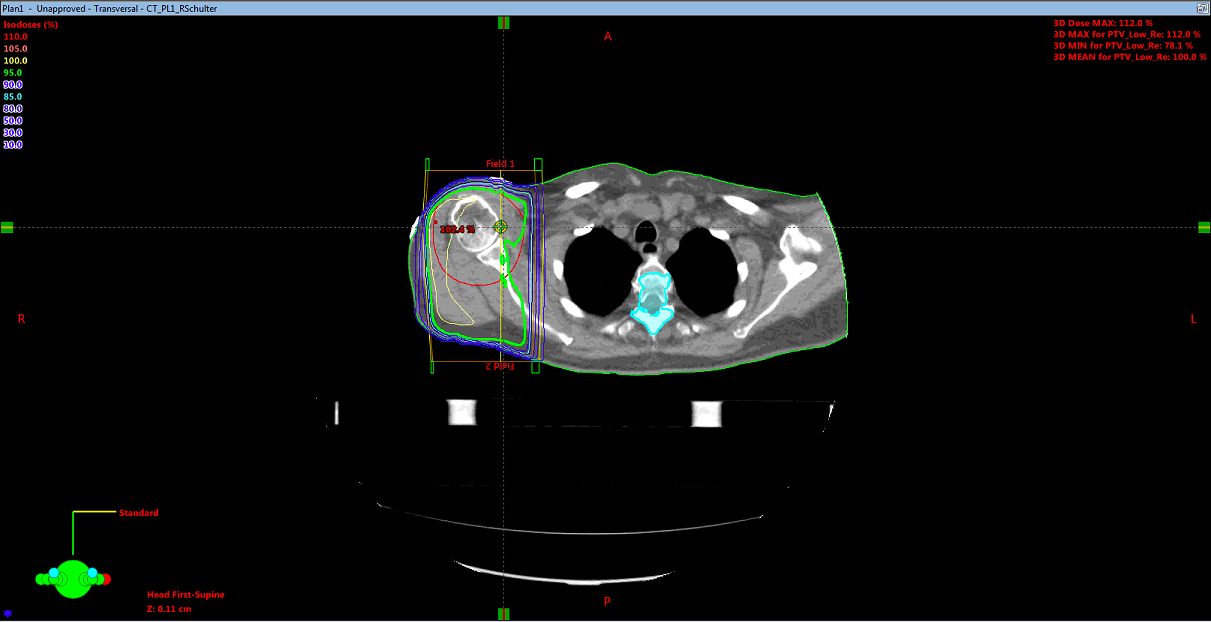
\includegraphics[width=\textwidth]{Bilder/SchulterZ.png}
  \caption{Darstellung der Dosisverteilung im Fuß in Transversalansicht.}
  \label{abb:Z}
\end{figure}

\begin{figure}[H]
  \centering
  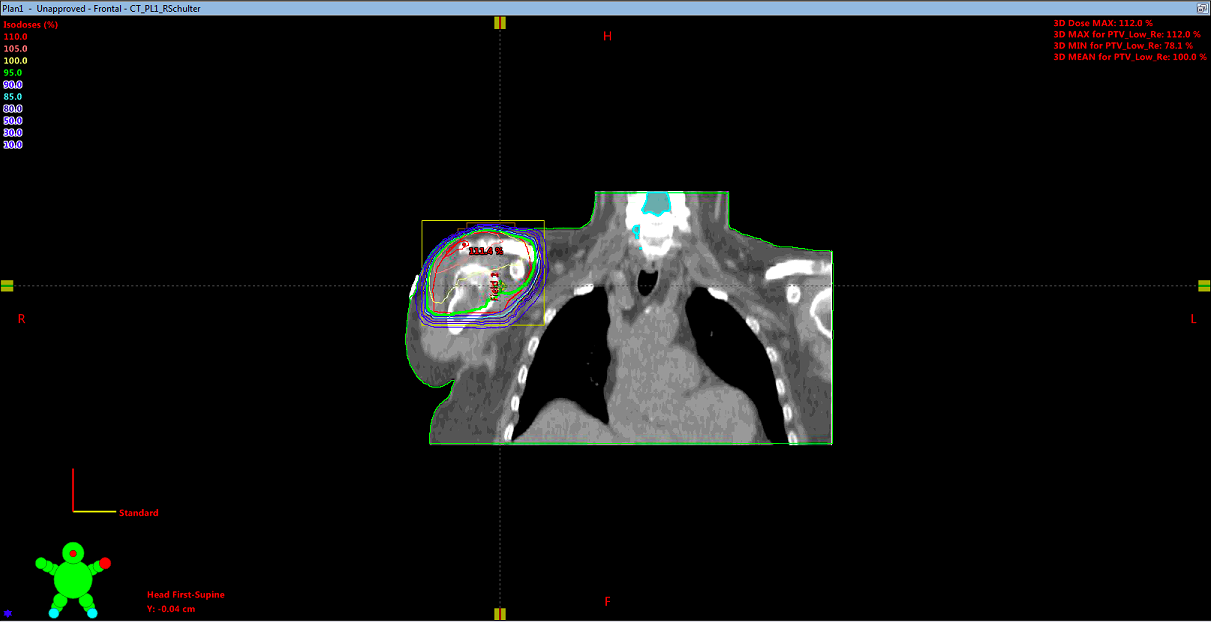
\includegraphics[width=\textwidth]{Bilder/SchulterY.png}
  \caption{Darstellung der Dosisverteilung im Fuß in Frontalansicht.}
  \label{abb:Y}
\end{figure}

\begin{figure}[H]
  \centering
  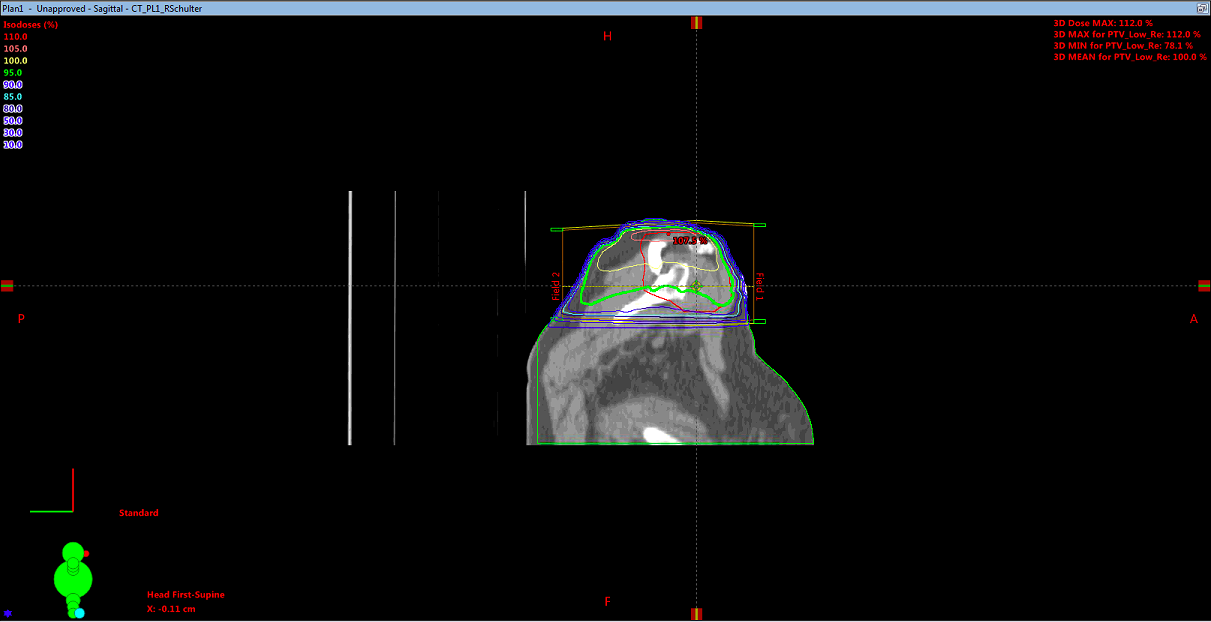
\includegraphics[width=\textwidth]{Bilder/SchulterX.png}
  \caption{Darstellung der Dosisverteilung im Fuß in Sagittalansicht.}
  \label{abb:X}
\end{figure}

Anhand der Dosisverteilung ist zu erkennen, dass es nicht komplett gelungen ist, das PTV mit
der $95\%$-Isodosenlinie zu umschließen. In den Bereichen des PTV, die tief innerhalb der Schulter liegen
ist nicht die gewünschte Dosis erreicht worden. Das liegt daran, dass in diesen Bereichen die Strahlungsfelder
durch Knochen, wie das Schlüsselbein oder das Schultergelenk, geschwächt werden und somit dort nicht die gewünschte Dosis deponiert werden kann.

Zur genaueren Beurteilung der Dosisverteilung ist das DVH in Abbildung \ref{abb:DVH} gezeigt.

\begin{figure}[H]
  \centering
  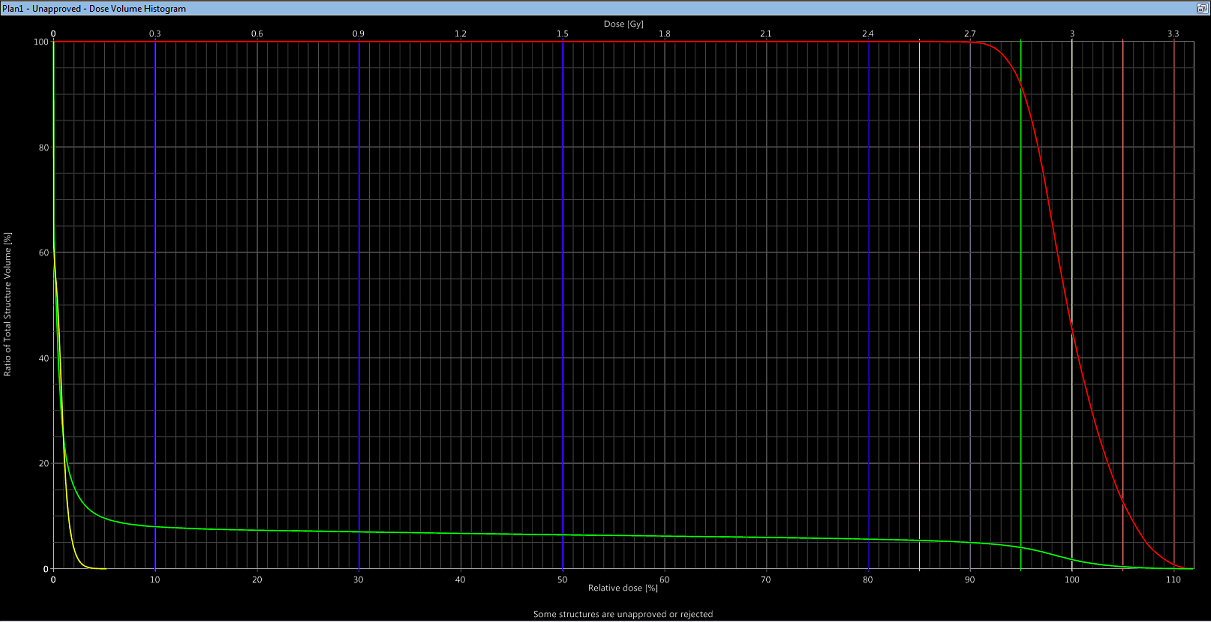
\includegraphics[width=\textwidth]{Bilder/DVH_SchulterEinzel.png}
  \caption{Dosis-Volumen-Histogramm für das PTV in rot und den gesamten Körper, der in dem CT-Bild abgebildet ist, in grün. Außerdem ist das DVH für die
  Lungen in gelb dargestellt.}
  \label{abb:DVH}
\end{figure}

Als erstes fällt auf, dass in nur einem sehr kleinen Teil der Lunge (gelbe Kurve) eine Dosis deponiert wird. Dabei ist die maximale relative Dosis
$5,2 \%$. Das bedeutet, dass die Strahlenbelastung der Lunge minimal ist.
Anhand der Kurve des PTVs (rote Kurve) ist zu erkennen, dass etwa $92\%$ des PTVs eine relative Dosis von $95\%$ erhält. Des weiteren Fällt auf,
dass die maximale relative Dosis $112\%$ ist. Diese Dosis liegt um $5\%$ über der erlaubten maximalen Dosis von $107\%$ \cite{ICRU}.
Allerdings wird die maximale Dosis nur in dem PTV deponiert und der Teil in dem die Dosis über $107\%$ liegt ist sehr klein, etwa $5\%$ des PTVs.
Die Stellen des PTVs, bei denen es nicht gelungen ist eine relative Dosis zu erreichen, erhalten
trotzdem mindestens eine Dosis von $78,1\%$. \\
Wird die Kurve des gesamten Körpers (grüne Kurve) betrachtet, ist zu erkennen, dass diese Kurve sehr schnell abfällt und nur etwa $20\%$ des
Körpervolumens eine relative Dosis von mehr als $1\%$ erhält. Insgesamt wird in dem gesamten Körper nur eine relativ geringe Dosis deponiert. \\

Durch die gewählte Feldkonfiguration kann gewährleistet werden, dass die gewünschte Dosisverteilung
in der Schulter weitgehend erreicht wird. Dabei handelt es sich um eine einfache Konfiguration
mit zwei opponierenden Feldern, die bei solchen Bestrahlungen völlig ausreichend ist um eine gute Dosisverteilung zu erzielen.
Weitere Felder hätten zu einer besseren Dosisverteilung,
bei der das PTV komplett von der $95\%$-Isodosenlinie umschlossen wird. Allerdings würde dadurch auch
die Dosis in gesunden Gewebe steigen und da sich viele Risikoorgane in unmittelbarer Nähe zu dem
PTV befinden ist dies nicht empfehlenswert.
